%%This is a very basic article template.
%%There is just one section and two subsections.

\documentclass[conference]{IEEEtran}



\usepackage{times}

% *** CITATION PACKAGES ***
%
\usepackage{cite}


% *** GRAPHICS RELATED PACKAGES ***
%
\ifCLASSINFOpdf
  \usepackage[pdftex]{graphicx}
\else
   \usepackage[dvips]{graphicx}
\fi


\usepackage[tight,footnotesize]{subfigure}
%\usepackage[caption=false]{caption}
%\usepackage[font=footnotesize]{subfig}



% *** PDF, URL AND HYPERLINK PACKAGES ***
%
\usepackage{url}
\usepackage[cmex10]{amsmath}


% correct bad hyphenation here
\hyphenation{op-tical net-works }


\begin{document}



\title{Image based Landmine detection}

%\section{Title}
% author names and affiliations
% use a multiple column layout for up to three different
% affiliations
\author{
\IEEEauthorblockN{Maha El Meseery}
\IEEEauthorblockA{Computer and Systems Department\\Electronic Research
Institute, Cairo, Egypt\\ Email: melmeseery@sci.eri.eg}
\and
\IEEEauthorblockN{Mahmoud fakhr el Deen}
\IEEEauthorblockA{Computer and Systems Department\\Electronic Research
Institute, Cairo, Egypt\\Email: mk@sci.eri.eg}
%\and
}
% make the title area
\maketitle


\begin{abstract}
%\boldmath
This paper presents a novel system for detection of landmines from
ground-penetrating radar (GPR) images.  A  multistatic ground-penetrating radar
(GPR) system produces scanning data of a several buried landmines on clean and
cluttered surfaces. The GPR time signal data is transformed into downcross
images of the soil and buried targets. Various image based techquies are used
to process these images to extract landmine characteristics.  A support
vector machine classifier (SVM) is used to identify the landmines from
the clutter and other buried objects in soil. The results show that the system
performe efficiently even in highly cluttered enviroment. % These images areprocessed

\end{abstract}
% IEEEtran.cls defaults to using nonbold math in the Abstract.
% This preserves the distinction between vectors and scalars. However,
% if the conference you are submitting to favors bold math in the abstract,
% then you can use LaTeX's standard command \boldmath at the very start
% of the abstract to achieve this. Many IEEE journals/conferences frown on
% math in the abstract anyway.

% no keywords




% For peer review papers, you can put extra information on the cover
% page as needed:
% \ifCLASSOPTIONpeerreview
% \begin{center} \bfseries EDICS Category: 3-BBND \end{center}
% \fi
%
% For peerreview papers, this IEEEtran command inserts a page break and
% creates the second title. It will be ignored for other modes.
\IEEEpeerreviewmaketitle
\section{Introduction}
\label{sec:introduction}
%%%%% firs some take %%% what is landmine detection \ldots.
One of most terrifying legacies of war that humanity faces is buired landmine
problem. Armed forces uses landmine  to destroy or disable enemy targets while
they pass over or near the landmine device. The problems rise after war and
armies move, the land continues to contains landmines for years. The
International Campaign to Ban Landmines (ICBL) \cite{ICBL2007} estimates that every year
there is more than 25,000 people killed or maimed by mines many of them are
children. A total estimate of 45-40 millions mines remains to be cleared
worldwoide \cite{ICBL2007}. One of the problems of mine removal or the demining is
high cost of the process. The cost of removing a single mine ranges from  300\$ to 1000\$
unlike the cost of laying a typical anti-personnel mine which ranges from 3\$ to
30\$.

Mines are usually made using metallic and non metallic materials and they in
general are either anti-presonal or anti-Tank mines. The use on non metallic
materials in manufacturing mines renders the conventional metal detector non
efficeints. Therefore researchers studied various other techniques to detect and remove landmines  \cite{Ho2002,Tan2005,Potin2006}.  Lately, several techniques in the area of sensor physics, signal processing, nano techonolgy and robotics were studied.  Ground penetrating radar (GPR), Infrared (IR), Sesiemic,  and ultrasound (US) sensors were developed and reviewed \cite{Scott2004,Ng2008}. These sensor usually generate a signal that requires different types of processing as noise removal, filtering, enhancement and feature extractions\cite{Ng2008,Potin2006,Wu2009}. Although systems can achieve high detection rates, they have done so at the expense of high false alarm rates.   % invistigated

 Two of the widely investigated sensor for mine detection are Ground-penetrating radar (GPR) and electromagnetic induction (EMI)  due to their complementary features. Detecting mines with low metal contents and moslty made of plastic is an advantage of GPR sensors over traditional metal detectors.  However, EMI sensors has better performance than GPR in detecting small antipersonal mines specially if they are bried deeply \cite{Frigui2010}. But some studies shows that even for the same sensor different algoritms can vary in perofromance for different mine types and soil conditions. For example, the system in \cite{Frigui2010}  presents an edge based feature that outperform a spectral detector in \cite{Ho2008} for the same antitank mine.

%   In fact, even for the same sensor, different detection algorithms may be more effective for different mine types, burial depths, and soil conditions . For instance, , it was shown that a detector that uses edge-based features \cite{Frigui2009} outperforms the spectral detector \cite{Ho2008} for antitank (AT) mines and shallow mines. On the other hand, the spectral detector outperforms the edge-based detector for weak scattering plastic mines \cite{Ho2008}. In [11], using a large GPR data set collected from four different sites, it was shown that the relative performance of four different detection algorithms is highly dependent on the site


The mine detection algorithm is similar to many automation and recognitio system, it has four main components: 1) reading sensor data 2) preprocessing 3) feature extraction and 4)classifier desing. The first step of any landmine system is reading and scanning the tested surface. After using the sensor to measure the input data, a preprocessing step focuses on normalizing data, correcting vaation and removal of stationary or latitude corrections. The next step, feature extraction, perform image or signal procesisng methods to extract the mine characterstics that are introduced to the last step which identify and localize the landemine.

The main contribution in this paper is using a simple image based feature to locate and detect mine from the GPR images. This paper introduce a landmine detection system that uses data collected from a multistatic Ground penetrating radar (GPR). The data are collected from scanning in x and y direction a clean and a highly cluttered stone surface using an array of resistive-vee antennas \cite{Counts2007} . This data are processed to genearate downcross image of ground at each x and y coordinate. An imaging algorithm similar to   \cite{Counts2007} is used to generate the ground model from the GPR.  After the ground images are obtained, the images are scanned using fixed window size to locate mine locations in the image. For each window in the scan a set of feature are extracted and preseneted to the classifier to identify it as clutter or mine.


The following section gives the details of the system; in Section  \ref{sec:gpr} a brief overview of GPR systems, section \ref{sec:system} gives a complete description of the system.  We presents the results and experiments in section \ref{sec:results} and we give the conclusion in section \ref{sec:con}.

% In  section  2  a  brief  history  for  mines  detection  is  introduced,  in  section  3,  a  complete  description  for  the  proposed  classification  algorithm  among  some  predefined  mine types is  demonstrated. In section  4 we present  and  discuss the results. In section 5 the work conclusion will be  given

\section{GPR Landmine Detection Overview}
\label{sec:gpr}
%Plain text.


%%%%%% what is the gpr system\ldots\ldots..
 Ground penetrating radar (GPR) is geophysical method that uses radar pulses to image the subsurface. It uses the principles of scattering electromagnetic waves to locate buried objeccts. An electromagnetic high frequency pulse is radiated from the transmitting antenna travels through the material with a velocity determined by the permittivity of the material. The wave travels in straight line downwards till it hit a surface with different permittivity and electrical properties from the surronding medium. If the wave hits a buried object, then part of the waves energy is “reflected” back to the surface, while part of its energy continues to travel downward. The recieving antenaa captures the reflected wave that traved to the surface,and recorded on a digital storage device for later interpretation.

The recorded data from the recieving antenaa over a period of time is called a “trace”. A trace is the time history of the travel single pulse from the transmit antenaa to the recieve antenaa. It include all the singal travel paths of all its different materials. The trace is the basic measurment of GPR surveys.  A scan is a trace where a color scale has been applied to the amplitude values. The round-trip (or two-way) travel time is greater for deep objects than for shallow objects. Therefore, the time of arrival for the reflected wave recorded on each trace can be used to determine the depth of the buried object, if the velocity of the wave in the subsurface is known. The principles of constructing a scan from a sequence of traces is shown in Figure \ref{figure:ScanA}.

 \begin{figure}
\centering
\label{figure:ScanA}
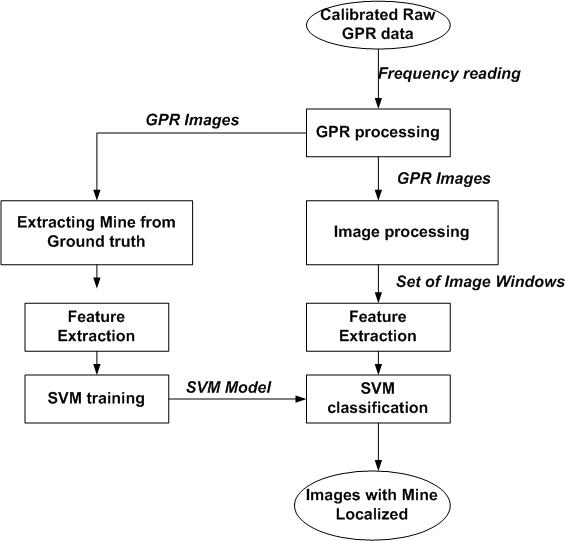
\includegraphics[width=0.25\textwidth]{images/BlockDiagram.jpg}
 \caption{Simple of an A scan }
\end{figure}
  %The wave that is reflected back to the surface is captured by a receive antenna, .The recieving antenaa detect the scattering of the wave from the buried object%The surface surrounding the advancing wave is called a wave- front. A straight line drawtn from the transmitter to the edge of the wavefront is called a ray. Rays are used to show the direction of travel of the wavefront in any direction away from the transmitting antenna.n.

% A typical GPR system has three main components: Transmitter and receiver that are directly connected to an antenna, and a control unit (timing) (Fig. 1). The transmitting antenna radiates a short high-frequency EM pulse into the ground, where it is refracted, diffracted and reflected primarily as it encounters changes in dielectric permittivity and electric conductivity.

% GPR data are displayed on printer paper or on a computer screen during acquisition (i.e., during real time). For a given transect, the data consist of a cross-section of signal amplitudes (intensities) versus location (along the two-way time axis and the horizontal axis). The intensity values are digitally recorded for each trace separately, converted back into analogue signals and displayed as signal voltage amplitude versus two-way time (the RAMAC GPR system uses a 16 bit A/D converter to convert the recorded signal to 65,536 levels of amplitudes). The plot is referred to as a normal-incidence time section (when the transmitter-receiver offset is negligible relative to the investigated depth and at a monostatic configuration). Simple processing is generally needed for a conventional display; otherwise, the display may become illegible. Such a typical processing is the running average of three to five samples along each trace plus the average of three traces along the profile in order to increase the signal to noise ratio. Amplifying gainis neededto increase the visibility of the deeper parts of the image. Basic processing routines can be applied during operation in the field while the image is built, in a way that does not affect the collected data.
% Ground penetrating radar (commonly called GPR) is a high resolution electromagnetic technique that is designed primarily to investigate the shallow subsurface of the earth, building materials, and roads and bridges. GPR has been developed over the past thirty years for shallow, high resolution investigations of the subsurface

% GPR uses the principle of scattering of electromagnetic waves to locate buried objects. The basic principles and theory of operation for GPR have evolved through the disciplines of electrical engineering and seismic exploration, and practitioners of GPR tend to have backgrounds either in geophysical exploration or electrical engineering. The fundamental principle of operation is the same as that used to detect aircraft overhead, but with GPR that antennas are moved over the surface rather than rotating about a fixed point. This has led to the application of field operational principles that are analogous to the seismic reflection method.


% The practical result of the radiation of electromagnetic waves into the subsurface for GPR measurements is shown by the basic operating principle that is illustrated in Figure A1. The electromagnetic wave is radiated from a transmitting antenna, travels through the material at a velocity which is determined primarily by the permittivity of the material. The wave spreads out and travels downward until it hits an object that has different electri- cal properties from the surrounding medium, is scattered from the object, and is detected by a receiving antenna. The surface surrounding the advancing wave is called a wave- front. A straight line drawn from the transmitter to the edge of the wavefront is called a ray. Rays are used to show the direction of travel of the wavefront in any direction away from the transmitting antenna. If the wave hits a buried object, then part of the waves energy is “reflected” back to the surface, while part of its energy continues to travel down- ward. The wave that is reflected back to the surface is captured by a receive antenna, and recorded on a digital storage device for later interpretation.
%
%
%
% 1-dimensional transmission line model for
% individual GPR A-scans is considered [6]. In transmission line mod-els for electromagnetic propagation, changes in the electromagnetic
% properties of transmission media are modeled as changes in the
% transmission parameters. Figure 1 shows a schematic of a hetero-geneous multi-layered soil with a buried object, and a simpli fi ed
% transmission line model for the corresponding GPR A-scan with
% characteristic impedances Z



% Ground-penetrating radar (GPR) is a geophysical method that uses radar pulses to image the subsurface. This nondestructive method uses electromagnetic radiation in the microwave band (UHF/VHF frequencies) of the radio spectrum, and detects the reflected signals from subsurface structures. GPR can be used in a variety of media, including rock, soil, ice, fresh water, pavements and structures. It can detect objects, changes in material, and voids and cracks.[1]
%
% GPR uses high-frequency (usually polarized) radio waves and transmits into the ground. When the wave hits a buried object or a boundary with different dielectric constants, the receiving antenna records variations in the reflected return signal. The principles involved are similar to reflection seismology, except that electromagnetic energy is used instead of acoustic energy, and reflections appear at boundaries with different dielectric constants instead of acoustic impedances.

% The depth range of GPR is limited by the electrical conductivity of the ground, the transmitted center frequency and the radiated power. As conductivity increases, the penetration depth decreases. This is because the electromagnetic energy is more quickly dissipated into heat, causing a loss in signal strength at depth. Higher frequencies do not penetrate as far as lower frequencies, but give better resolution. Optimal depth penetration is achieved in ice where the depth of penetration can achieve several hundred meters. Good penetration is also achieved in dry sandy soils or massive dry materials such as granite, limestone, and concrete where the depth of penetration could be up to 15 m. In moist and/or clay-laden soils and soils with high electrical conductivity, penetration is sometimes only a few centimetres.
\section {System Overview}
\label{sec:system}


This work presents a system that uses image based analyis to extract mine features from GPR images. Figure \ref{fig:block}
shows the block digram of the system. The first block in generating the scan images form the calibrated data from the GPR antnna. After images are comptued the images are scanened fixed size windows to locate the mines. For each window a set various feature extraction method is used to obtain a feature vector that will be used in classification. A SVM classifier is ued to identify if the window represents a mine or not.  %The training of SVM classifier is provided directly from a the GPR scan images.
 \begin{figure}
\centering
\label{fig:block}
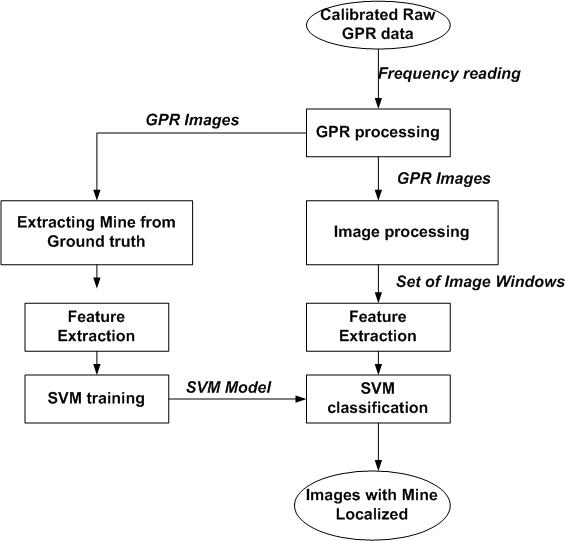
\includegraphics[width=0.45\textwidth]{images/BlockDiagram.jpg}
 \caption{The Block diagram }
\end{figure}

The follwoing section gives more details on each block of the system.

\subsection{GPR processing}

A multistatic ground-penetrating radar (GPR) presented in \cite{Counts2007} used to measure the response of a
number of targets to produce data for the investigation of  the system. The system consist of linear arry of resistitve vee antennas. The array has two transmitters and four receivers which provide eight bistatic spacings from 12 to 96 cm in 12-cm increments. The sysstem scans a surface that contained buried targets with and without surface clutter (layer of rocks ).  The measured responses are calibrated so that the direct coupling in the system is removed, and the signal reference point is located at the antenna drive point.

The GPR antenaa scans a region of  1.8x1.8 m  at a certain higth above the surface \cite{Counts2007}. Figure \ref{fig:mineshapes} shows various types of mine buried in the location specified by figure \ref{fig:minloc}. The scan is reference by x and y coordinate ranging from -90 to 90 using 2 cm increments.

 \begin{figure}
\centering
\label{fig:minloc}
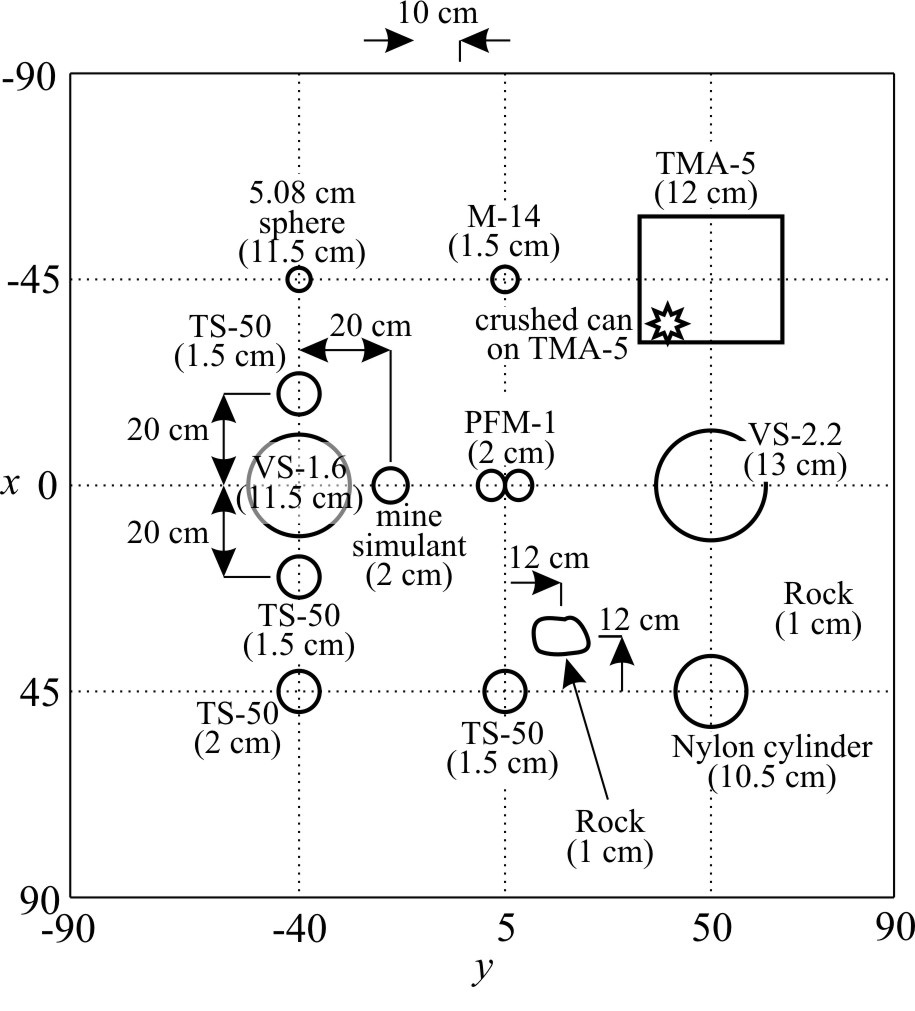
\includegraphics[width=0.35\textwidth]{images/MineLocations.jpg}
 \caption{Mine Locations}
\end{figure}

 \begin{figure}
\centering
\label{fig:mineshapes}
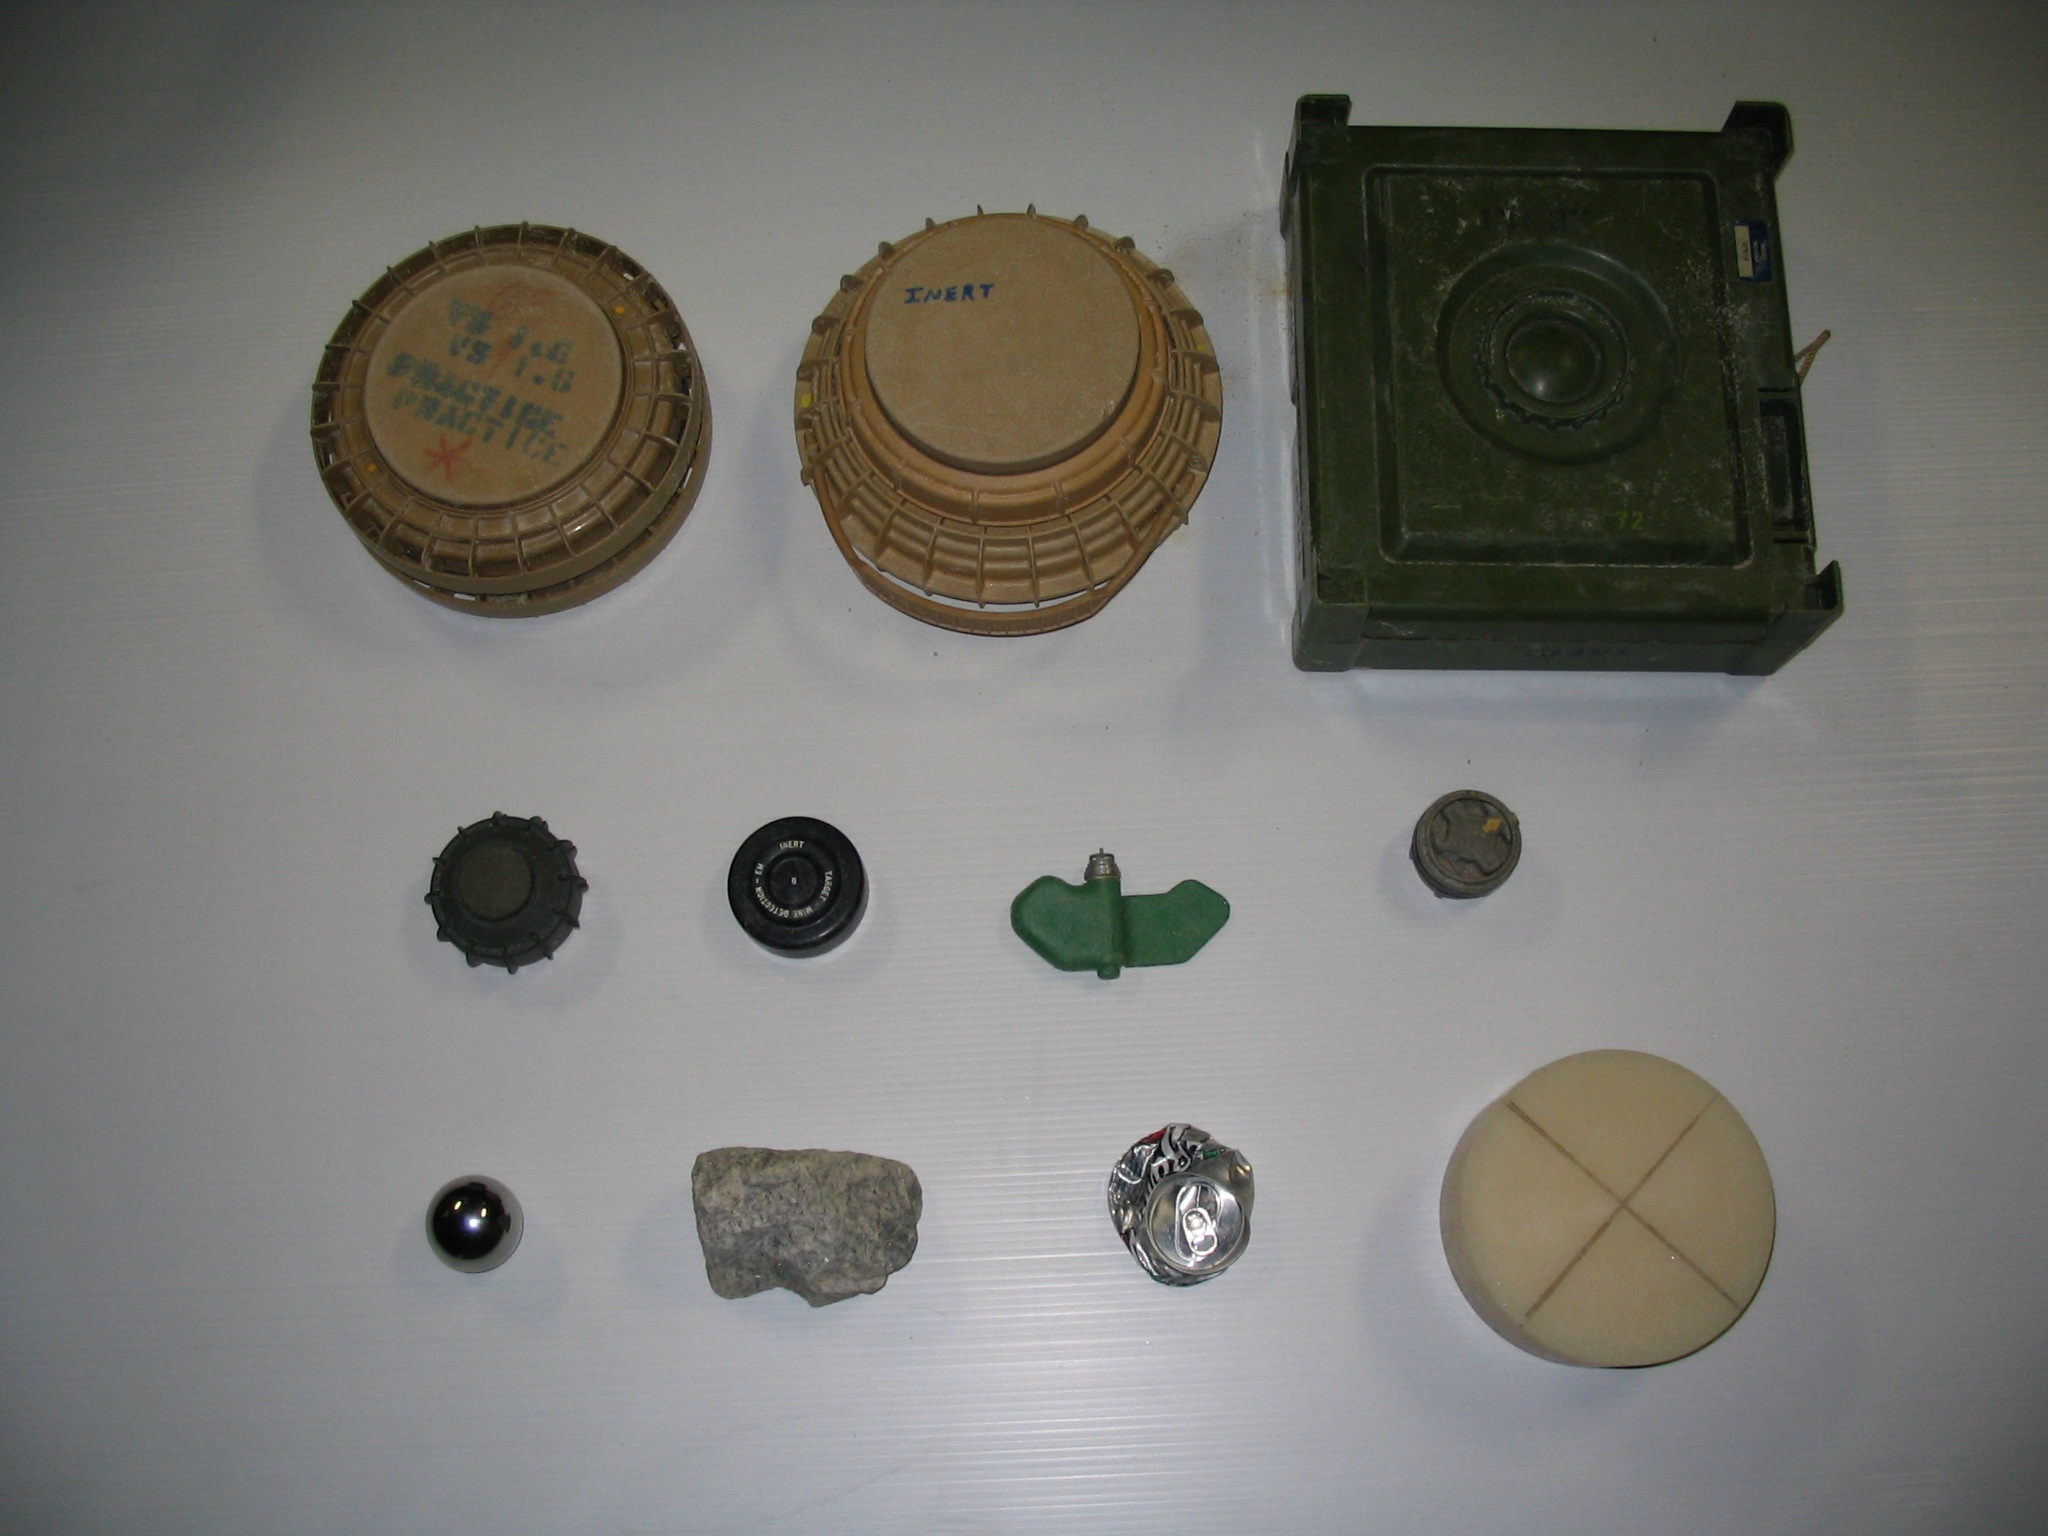
\includegraphics[width=0.35\textwidth]{images/MineShapes.jpg}
 \caption{ Sample of mines  }
\end{figure}

The data calibrated according were stored in Matlab file format. Each Matlab file contains one set of measured and calibrated data obtained from a single scan of 1.8 x 1.8 m region. The stored variables are responses from eight bistatic spacings (401 x 91 x 91 double precision), frequency points at which the data are measured (401 x 1 double precision), and x- andy -coordinates of each measurement (91 x 1).



I took the frequency measure data and converted them to time domain using inverse fourier transorm. Figure \ref{figure:ScanA} shows a single time signal for a specific x- and y- coordinate. A 2D image is generated form scannign the data in x direction and concatenating time signals in y-directions. Figure \ref{fig:mineAtx0} shows the dB scale of the image comuted x =0 , the location of TM1 and VS1 mine are clear in the image. % adding To generate a For each x- and y- coordiante the data generate a time sigal that can  be used to model the soil and subsurface objects








 \begin{figure}
\centering
\label{fig:mineAtx0}
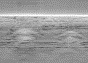
\includegraphics[scale=1.5]{images/MineCleanX0.jpg}
 \caption{The 2D scan Image at x =0 }
\end{figure}

\subsection{Image processing}
\label{sec:image}

The system test various image based method to investigate the best feature extraction to characterize mines in the GPR images. A fixed size window with no overlap is used to scan the gpr images. Several imaga analysis methods are used to extract features and used to compare to achieve the best performance. The next section explain each feature in details.

\subsubsection {Gradient Features}
\label{sec:grad}
To extract gradient features \cite{Liu2003}, the gradient operator is first applied to the gray-scale image of the digit to give two gradient components: strength $|g(x,y)|$ and direction $\angle g(x,y)$ at each point $(x,y)$ of the image $f$. This is done by applying Sobel operator \cite{gonzales2002} on the image to extract vertical and horizontal gradient components. Then the gradient strength and direction is extracted using equations \ref{eq:1} and  \ref{eq:2}, respectively,

\begin{equation}
|g(x,y)|=\sqrt{g^{2}_{x}(x,y)+g^{2}_{y}(x,y)}
\label{eq:1}
\end{equation}
\begin{equation}
\angle g(x,y)=\tan^{-1} \frac{g_{y}(x,y)}{g_{x}(x,y)}
\label{eq:2}
\end{equation}
where $g_{y}(x,y)$ and $g_{x}(x,y)$ are the vertical and horizontal gradient components extracted from Sobel operator.

The gradient vector $g(x,y)$ (expressed as strength strength $|g(x,y)|$ and direction $\angle g(x,y)$  at each point $(x,y)$ of the image is then decomposed into the 8 Freeman\cite{gonzales2002} directions shown in Figure \ref{fig:freeman} . The gradient vector is decomposed into the 8 Freeman directions by projecting the vector into the nearest two Freeman directions as shown in Fig. 3.
The gradient features are composed of 8 layers; each corresponding to one of the Freeman directions. Each layer is the projection of the gradient vectors of the image into the corresponding Freeman direction.

 \begin{figure}
\centering
\label{fig:freeman}
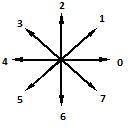
\includegraphics[scale=0.55]{images/freemanCodes.jpg}
 \caption{The 2D scan Image at x =0 }
\end{figure}


% A Gaussian mask h(x,y) is then applied to each layer,
%
%
% and then the layers are uniformly sampled to give 5×5 measurements. The parameter σ is related to the sampling interval t via the empirical relation  [3]. This means that the gradient features are composed of 8×5×5 = 200 elements. The gradient feature extraction technique is very powerful as shown in [3] and as will be shown in the results section (section 5) of this paper.
\subsubsection {Kirsch Features}
The Kirsch features \cite{Liu2003} are extracted by decomposing the image into 4 layers corresponding to 4 edge orientations: horizontal ($g_h$), vertical ($g_v$) , right diagonal ($g_{rd}$), and left diagonal ($g_{ld}$). These layers are extracted by applying Kirsch masks on the image,
\begin{equation}
 g_h=\max \left( |f*k_{h1}| , |f*k_{h2}| \right)
\label{eq:kirsh1}
\end{equation}
\begin{equation}
 g_v=\max \left( |f*k_{v1}| , |f*k_{v2}| \right)
\label{eq:kirsh1}
\end{equation}
\begin{equation}
 g_{rd}=\max \left( |f*k_{rd1}| , |f*k_{rf2}| \right)
\label{eq:kirsh1}
\end{equation}
\begin{equation}
 g_{ld}=\max \left( |f*k_{ld1}| , |f*k_{ld2}| \right)
\label{eq:kirsh1}
\end{equation}
where $*$ denotes 2D convolution operation \cite{gonzales2002}, $kh1$ and $kh2$ are Kirsch masks responsible for extracting horizontal edges, $kv1$ and $kv2$ for horizontal edges, $krd1$ and $krd2$ for right diagonal edges, and $kld1$ and $kld2$ for left diagonal edges. Figure \ref{fig:kirshMasks} shows all Kirsch masks.

  \begin{figure}
\centering
\label{fig:kirshMasks}
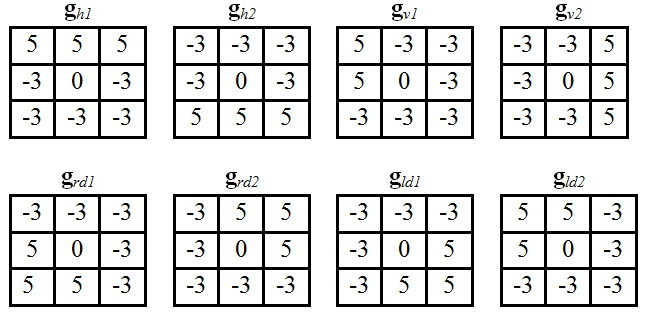
\includegraphics[width=0.40\textwidth]{images/kirshAll.jpg}
 \caption{The 2D scan Image at x =0 }
\end{figure}


%A Gaussian mask is then applied to all the 4 layers and 5×5 measurements are extracted from each of them in the same manner done with gradient features (section 4.1). This means that Kirsch features are composed of 4×5×5=100 elements.
\subsubsection {Local Chain Code Features}

To extract the local chain code features \cite{Zhang2004}, the contour of the digit is first followed by any contour following algorithm, and then each contour point of the image is marked with the corresponding Freeman direction. The image is then decomposed into 8 layers; each layer contains only contour points that belong to the corresponding Freeman direction. Each of the 8 layers is then uniformly partitioned into 5\times5 zones.


\subsubsection {Wavelet Features}

Wavelet transform \cite{gonzales2002} is best known for extracting essential infromation contained in a signal or an image. This reduce the dimensionality of the features and leads to faster classification. It also reduces the noise and the non-essential information that may confuse the classifier.  Wavelet tranform could be applied to an image or to the gradient decomposition of an image.  We use the former method

Wavelet transform \cite{gonzales2002} extracts the essential information contained in a signal or image. This may help in reducing the dimensionality of the problem which leads to faster classification. Also it might reduce the noise and the non-essential information that may confuse the classifier leading to better classification performance. Wavelet transform could be applied on the image directly or could be applied on the gradient decomposition of the image. In our study, we applied the former method. The image is first resized to be $64\times64$ and then the image is composed into 3 resolution levels. The 3rd level approximation of the image (which is a $8\times8$ image) is then used as features.


\subsubsection {Concatenation of low dimensional features}
\label{sec:conLow}
A concatentaion of 6 low dimentional feature are used to form a single feature vecotr. Any single feature is not effective but their concatenation proved to produce a set of  powerful features.   Each of the 6 low dimensional feature families is going to be discussed in the following subsections.



\begin{enumerate}
  \item Raw Image Zoning \\
  The image is divided into $5\times5$ zones and the average of raw pixel values of each zone is calculated leading to a feature vector of 25 elements\cite{Trier1996}.

	\item Vertical and Horizontal Projections \\
	The histogram of the horizontal and vertical projections is used as a feature vector \cite{Trier1996}

	\item Vertical and Horizontal Cross Counts \\
	The first step is binarizing the image and then computing the number of crossing from 0 to 1 and vice-versa in  both the hrozintal and vertical direction. The number of cross counts in each direction is used as the feature vector . %The image is first binarized, and then the vertical and horizontal cross counts are calculated leading to the feature vector.
	\item  Centroidal Distances \\
	The image is divided into 16 anglar sector from the image center of gravity. The centroid of each sector is calculated and the distance between the image centeroid and the sector centroid is normalized by dividing them by the bounding box diameter\cite{ElSherif2007}.  The normalized distances are used as the feature vector.
% 	In this technique , the digit image is partitioned into 16 sectors around the digit center of gravity (the centroid) as shown in Figure 5. Then the centroid of each sector are calculated. The distances between the whole digit centroid and sectors centroids are calculated and normalized by dividing them by the digit bounding box diameter. This forms a 16-element feature vector.

\item Directional Features\\
The directional features are formed as follows \cite{ElSherif2007}. A 4-element vector is used to label each background pixel. To label each background pixel, we walk upward and if we face a foreground pixel, the first element of the 4-element vector is set to 1, otherwise we set it to 0. Next we walk right till we find a foreground pixel, the second element is set to 1 otherviwse set it to 0. The remaining elements are filled in the same mannar till all 4 prinicipal directions are processed. After all directions for all background pixels are labeled, the combination of 4-element vector is marked and ecah combination is labedl with a different label. Hence, we have 16 different labels which we compute the histogram of each label and use as feature vector.

% Each background pixel is labeled by a 4-element vector. For each background pixel we walk upward; if a foreground pixel is found, the first element of the 4-element vector is set to ‘1’ otherwise set to ‘0’.
%  Then we walk to the right; if a foreground pixel is found,
%  the second elements is set to ‘1’ otherwise set to ‘0’; and so on till we finish the 4 principal directions.
%
%  Then for each combination of 0’s and 1’s in the 4-element vector, we give a different label. Hence, we have 16 different labels. Now each of foreground pixels has one label of the 16 labels. The final feature vector is the histogram of such labels giving rise to a 16 element feature vector.
\item Length-Normalized Contour \\
The normalized contour is computed form the horizontal and vertical coordinates of the boundary pixels as mentioned in  \cite{ElSherif2007}. The first step is extracting the boundry of a shape using a contour following algorithm. The extracted boundry point is stored by both its horizontal and vertical coordinates.  The horizontal locations are magnitude-normalized by dividing the width of the bounding box. Simillary, the vertical locations are normalized by dividing them by the height of the bounding box. The average of 10 different portions of both the horizontal and vertical locations represent the feature vector. %portions Both the horizontal and vertical locations are partitioned into 10 different portions. The average of each portion is calculated and % is used to normalized the horizontal locations by dividing

%In this technique \cite{ElSherif2007}, the horizontal and vertical coordinates of the boundary pixels of the digit are used as features. First, the boundary of the digit is extracted using a contour following algorithm; then, each boundary point is stored by its horizontal and vertical coordinates. Horizontal locations are magnitude-normalized by dividing them by the width of the digit bounding box. Vertical locations are also magnitude-normalized by dividing them by the height of the bounding box. Then both horizontal and vertical locations are partitioned into 10 portions and the average of each portion is calculated leading to a feature vector of length 20.

% Feeding the classifier with the concatenation of different features without any preprocessing step would lead to very bad results because features of large magnitudes will dominate. Hence, we applied mean and variance normalization [14] to all the low-dimensional features discussed in this section before concatenating them into a feature vector of length 156.

\end{enumerate}
% \subsubsection {Local Directional Features}
% Local directional features extraction is a novel technique that we present in this paper. It is a natural extension of the directional features presented in section \ref{sec:conLow}  Like directional features, each background pixel is labeled by a 4-element vector which leads to 16 different labels. However not all labels are used. Only 9 labels corresponding to 9 situations are considered: (1) closed from all directions (i.e. black pixel can be reached when moving in all the principal 4 directions), (2) open up (i.e. black pixel can be reached when moving in the principal 4 directions except when moving upward), (3) open down, (4) open right, (5) open left, (6) open up and right, (7) open up and left, (8) open down and right, and (9) open down and left.
%
% The image is then decomposed into 9 layers; each layer corresponds to one of the 9 labels. Pixel $(x,y)$ in layer #n is illuminated only if pixel $(x,y)$ in the image has been given the label #n. A Gaussian mask is then applied to all the 9 layers and 5x5 measurements are extracted from each of them in the same manner done with gradient features (section \ref{sec:grad}).

% \subsubsection {Moments}
% The orthoganal moments of the $7^th$ order are computed for each block of the image
\subsubsection {Discrete cosine transform}
The Discrete cosine transform for each block is computed and the return the higher order features only are used as features.

\subsection {Classification}
A single Binary Support vector machine (SVM) classifier is used to classify the extracted feature.  As shown in figure \ref{fig:minloc} the x, y  coordinate and burial depth is given for all mines. This infromation is used to extract samples for the trainging. Regions of mine locations  are extracted from the scan image data and used to trained the SVM classifier to the mine features. Random clutter location are also extracted and feature were comtued and present to be trained the SVM classifier.  Eventhough that mine dection can be viewed as a single class problem tests shows that considering the problem as two classes problem where first class is mine and second is clutter  achieve better results.

The testing are genearted by scanning the image using a fixed window which is used to divide the input scan image into a set of equal windows. Each window, which either represents a clutter or a mine location, feature vector is represented to the svm classifier. The classifier then labels each window in the image using either mine or clutter label.
  %The training is set iThe location of all mines in scan image areThe location of the The training set is generated from

\section{Experiments}
\label{sec:results}

As mentioned before the training set of the system are extracted from the mine location in GPR images and used as input for training the classifier. The different clean and rock data are used to provide differiance in training and testing. In all the present results, the average of two different experiments spliting data into training and testing are provided. In the first experiment the training data are extracted from clean surface data and tested on cluttered rock surface data. The second experiment, extracts the training data from the rock surfaced data and tested on clean surface images. The recognition rate is computed as the number of correct identified samples from the images windows over total number of samples.
 \subsection{Effect of Feature extraction method}

Different feature extraction method explained in sections \ref{sec:image} were used to locate the buried landmines. Figure \ref{fig:ResultsFeats} shows the results of using the different feature extraction methods. The results show that the Local chain code and gradient features achieve the best recognition rate. Local chain code features outperform the gradient feature in term of computaional complexity.  The results reveal that local features and structures outperform global featurs like (Discrite cosine transform) DCT.

   \begin{figure}
\centering
\label{fig:ResultsFeats}
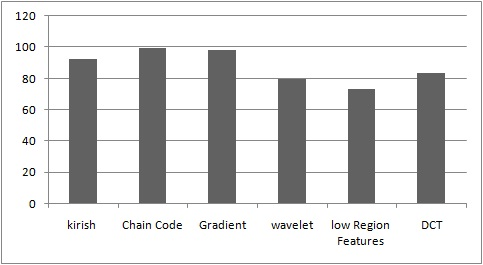
\includegraphics[width=0.45\textwidth]{images/ResultsFeats.jpg}
 \caption{Recongnition rate of different feature extraction methods }
\end{figure}
 %  the testing set  must be different than the training set,
\subsection{Effect of vairous window size}
We conducted several experiments on the best scan window size. The scan window specify the size of the window tested by the classifier. Figure \ref{fig:ResultSize} displays the result of differnet window size from 5 to 15 pixel in width and height. the results shows that the system achieved best performance with the smallest window size, 5x5 pixels, this is understandable with respect to the size of the buried mines.  The size of the targets buried which varies from    5 X 4 cm  TS-50 antipersonnel (AP)  mine  to 22X9 cm VS-1.6 antitank (AT) mine. The small window provide more detailed features for local features and provide better charactersitc for mines.   % smaller the window t  %The size of the scan window
%Different feature extraction method explained in sections \ref{sec:image} were used to locate the buried landmines. Figure \ref{fig:ResultsFeats} shows the results of using the different feature extraction methods. The results show that the Local chain code and gradient features achieve the best recognition rate. Local chain code features outperform the gradient feature in term of computaional complexity.  The results reveal that local features and structures outperform global featurs like (Discrite cosine transform) DCT.
  \begin{figure}
\centering
\label{fig:ResultSize}
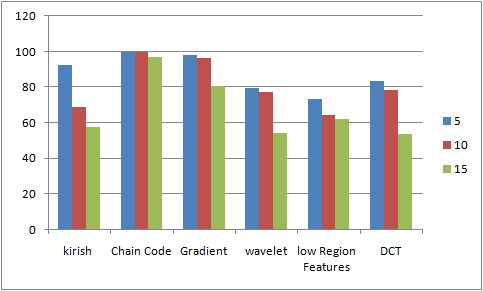
\includegraphics[width=0.45\textwidth]{images/ResultSize.jpg}
 \caption{Recongnition rate of different scan window sizes}
\end{figure}


 \subsection{Effect of Mine vs. Clutter}

 The output of the system is a map of location of targets landmine to the locaion of the clutter in the GPR images. Figure \ref{fig:ResultMineClean} shows the ouput of the GPR images with the location of the mine idetified by the Red rectangle the remaiing locations were marked as clutter and ignored by the system.The actual location of mine are marked by while rectangles. Figure \ref{fig:ResultMineRock} shows similar results with subsurface target with the rocks on the surface. The results shows the efficiency of the system and low false alarm rate.


  \begin{figure}
\centering
\label{fig:ResultMineRock}
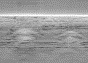
\includegraphics[width=0.25\textwidth]{images/MineCleanX0.jpg}
 \caption{Recongnition rate of different scan window sizes}
\end{figure}
  \begin{figure}
\centering
\label{fig:ResultMineClean}
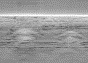
\includegraphics[width=0.25\textwidth]{images/MineCleanX0.jpg}
 \caption{Recongnition rate of different scan window sizes}
\end{figure}


\section {Conclusion}
\label{sec:con}
This paper presente a simple image based method to detect landmine from GPR images. The image based feature uses different features methods to generate the best recognition rate for landmine detection system. The system achieved high recognition rate in clean and highly cluttered surfaces. The results shows the system can be easily applied to output of GPR systems with  mininum number of processing . The best feature extraction method used was local concavity of image which achieved 98\% recognition rate in both cluttered and clean surface data.




%develop new features based on structural information.
\bibliographystyle{IEEEtran}
\bibliography{library,Landmine}
\end{document}
